\documentclass[10pt]{article}

\usepackage[margin=2.4cm]{geometry}
\usepackage{amsmath, amssymb, bm}
\usepackage{booktabs}
\usepackage{graphicx}
\usepackage{algorithm}
\usepackage{algpseudocode}
\usepackage{tikz}
\usetikzlibrary{positioning, arrows.meta, fit, backgrounds, calc}
\usepackage[colorlinks=true, linkcolor=blue, citecolor=blue]{hyperref}
\usepackage{enumitem}
\setlist{itemsep=1pt, topsep=2pt}

\newcommand{\sg}{\operatorname{sg}}
\newcommand{\cossim}{\operatorname{cos}}
\newcommand{\xhat}{\hat{x}_0}
\newcommand{\xtil}{\tilde{x}_0}
\newcommand{\ftext}{\bar{f}_{\mathrm{text}}}
\newcommand{\fimg}{\bar{f}_{\mathrm{img}}}

\title{\textbf{Encoder-Scored Self-Distillation for Prompt--Image Alignment\\in Flow-Matching Text-to-Image Models (v5)}}
\author{EnergyVLM}
\date{\today}

\begin{document}
\maketitle

\begin{abstract}
We fine-tune Stable Diffusion 3.5--Medium to improve prompt--image alignment
\emph{without} a reward-model network and without a standard diffusion loss on
real images. A frozen-in-structure EMA teacher generates short
classifier-free-guided denoising trajectories; the trainable student is asked
to be \emph{consistent} with the teacher across an asymmetric timestep gap
(student at a noisier state must predict the teacher's cleaner-state Tweedie
estimate). Trajectory--timestep pairs are importance-weighted by a Boltzmann
distribution over a learned CLIPScore proxy: a small co-trained projector maps
predicted clean latents directly into CLIP space, where they are scored
against the \emph{caption's} text embedding. An explicit reward term and a
real-image anchor for the projector complete the objective.
\end{abstract}

\section{Method}

\paragraph{Setup.}
Let $v_\theta$ denote the SD3.5-M MMDiT velocity network (the
\emph{student}, trainable) and $v_\xi$ its exponential moving average (the
\emph{teacher}, frozen per step):
\begin{equation}
\xi \leftarrow m\,\xi + (1-m)\,\theta, \qquad m = 0.999 .
\label{eq:ema}
\end{equation}
Both operate in the VAE latent space ($16 \times 64 \times 64$ at $512^2$).
A projector $g_\phi$ (REPA-style 3-layer MLP, $16 \to 2048 \to 2048 \to 768$
as $1{\times}1$ convolutions with parameter-free GroupNorm input
normalization, global mean pooling) maps latents into the CLIP joint
text--image embedding space. A frozen CLIP ViT-L/14 provides two kinds of
targets: the \emph{text} embedding $\ftext$ of the training caption (computed
per step by the text tower) and the \emph{image} embedding $\fimg$ of the
paired real COCO image (precomputed once and cached). DINOv2 is supported as
a legacy alternative encoder.

\paragraph{Pass 1: teacher rollout (no grad).}
For one caption $c$ per step, the teacher generates $N$ trajectories from
Gaussian noise with $K$ Euler steps of the flow-matching ODE under
classifier-free guidance (CFG):
\begin{equation}
v^{\mathrm{cfg}}_\xi = v_\xi(z_k, t_k, \varnothing)
  + \omega \big( v_\xi(z_k, t_k, c) - v_\xi(z_k, t_k, \varnothing) \big),
\qquad
z_{k+1} = z_k + (\sigma_{k+1} - \sigma_k)\, v^{\mathrm{cfg}}_\xi .
\end{equation}
At every index $k$ in the scoring window
$\mathcal{K} = \{ \lceil 0.4K \rceil, \dots, \lfloor 0.9K \rfloor \}$ the
teacher's Tweedie estimate is cached from the \emph{CFG-mixed} velocity
(guidance distillation):
\begin{equation}
\xtil^{(i,k)} = z^{(i)}_k - \sigma_k\, v^{\mathrm{cfg}}_\xi\big(z^{(i)}_k, t_k, c\big).
\end{equation}
No additional teacher forwards are needed afterwards.

\paragraph{Pass 2: asymmetric student prediction (single batched forward).}
For each $k \in \mathcal{K}$ a gap $\Delta_k \sim \mathcal{U}\{1, \dots, 3\}$
is drawn (one per $k$, shared across trajectories). The student is evaluated
at the \emph{noisier} state $z_{k - \Delta_k}$ of the same trajectory, and all
$|\mathcal{K}| \cdot N$ pairs are concatenated into one batched forward:
\begin{equation}
\xhat^{(i,k)} = z^{(i)}_{k-\Delta_k}
  - \sigma_{k-\Delta_k}\, v_\theta\big(z^{(i)}_{k-\Delta_k},\, t_{k-\Delta_k},\, c\big).
\end{equation}
Since $z_k$ is reached from $z_{k-\Delta_k}$ by teacher Euler steps, both
predictions estimate the same trajectory endpoint: this is consistency
distillation in $x_0$ space across an asymmetric timestep gap.

\paragraph{Scoring and Boltzmann weighting.}
Each student prediction is scored in CLIP space against the caption:
\begin{equation}
s_{i,k} = \cossim\big( g_\phi(\xhat^{(i,k)}),\; \ftext \big)
\qquad \text{(a learned CLIPScore proxy).}
\end{equation}
Importance weights form a product of two Boltzmann distributions with energy
$E = -s$ (temperatures $\tau_N, \tau_K$), \textbf{detached} from the graph:
\begin{equation}
w^{\mathrm{traj}}_i = \frac{\exp\!\big(\bar{s}_i / \tau_N\big)}{\sum_{i'} \exp\!\big(\bar{s}_{i'} / \tau_N\big)},
\quad
w^{\mathrm{step}}_{i,k} = \frac{\exp\!\big(s_{i,k} / \tau_K\big)}{\sum_{k'} \exp\!\big(s_{i,k'} / \tau_K\big)},
\quad
W_{i,k} = \sg\!\big[ w^{\mathrm{traj}}_i \cdot w^{\mathrm{step}}_{i,k} \big],
\end{equation}
where $\bar{s}_i = \tfrac{1}{|\mathcal{K}|}\sum_k s_{i,k}$, and the scores
entering each softmax are \emph{standardized along that softmax's axis}
(mean $0$, variance $1$). Raw CLIP cosines spread only a few hundredths
across samples of one prompt, which would leave $\mathrm{softmax}(s/\tau)$
near-uniform for any reasonable raw $\tau$; z-scoring makes $\tau$ a
scale-free selectivity knob (verified via the logged weight entropies).
Gradient flow through the softmax weights is deliberately blocked: it would
reward routing mass onto the easiest pairs, i.e.\ \emph{lowering} $s$ exactly
where matching is hard. Detached, $W$ is a self-normalized
reward-weighted-regression weight (soft best-of-$N$): well-aligned
trajectories and timesteps dominate the consistency target.

\section{Objective}

\begin{equation}
\boxed{\;
\mathcal{L} =
\underbrace{\sum_{i,k} W_{i,k}\;
  d\big( \xhat^{(i,k)},\, \sg[\xtil^{(i,k)}] \big)}_{\mathcal{L}_{\mathrm{cons}}\;\text{(weighted consistency)}}
\;+\; \lambda_r
\underbrace{\frac{1}{N |\mathcal{K}|} \sum_{i,k} \big( 1 - s_{i,k} \big)}_{\mathcal{L}_{\mathrm{reward}}\;\text{(alignment reward)}}
\;+\; \lambda_a
\underbrace{\Big( 1 - \cossim\big( g_\phi(\mathcal{E}(x_{\mathrm{real}})),\, \fimg \big) \Big)}_{\mathcal{L}_{\mathrm{align}}\;\text{(projector anchor)}}
\;}
\end{equation}

\begin{itemize}
\item $\mathcal{L}_{\mathrm{cons}}$ uses the dimension-scaled pseudo-Huber
metric (iCT), robust to outlier pairs produced by aggressive gaps:
$d(a, b) = \sqrt{ \lVert a - b \rVert_2^2 + c^2 } - c$ with
$c = 0.00054 \sqrt{D}$, $D = 16 \cdot 64 \cdot 64$ ($c \approx 0.14$).
\item $\mathcal{L}_{\mathrm{reward}}$ is the \emph{only} path through which
the alignment score reaches the student (ReFL-style, but through the cheap
projector proxy instead of a decoded-image reward):
$\mathcal{L}_{\mathrm{reward}} \to s \to g_\phi(\xhat) \to v_\theta$.
\item $\mathcal{L}_{\mathrm{align}}$ regresses the projector on the VAE
latent $\mathcal{E}(x_{\mathrm{real}})$ of the paired real image toward its
CLIP \emph{image} embedding. It anchors $g_\phi$ as a faithful latent-space
image encoder, so the reward cannot be satisfied by a projector that
collapses toward the text-embedding direction. The student receives no
gradient from this term.
\end{itemize}
After each optimizer step the teacher is updated by Eq.~\eqref{eq:ema}.
Algorithm~\ref{alg:v5} summarizes one training run.

\begin{algorithm}[t]
\caption{Encoder-Scored Self-Distillation (v5)}
\label{alg:v5}
\begin{algorithmic}[1]
\Require pretrained flow-matching model $v_{\theta}$; frozen CLIP text/image
  towers, frozen VAE $\mathcal{E}$; dataset
  $\mathcal{D} = \{(x_{\mathrm{real}}, c)\}$;
  trajectories $N$, rollout steps $K$, scoring window $\mathcal{K}$,
  max gap $\delta_{\max}$; temperatures $\tau_N, \tau_K$;
  weights $\lambda_r, \lambda_a$; EMA decay $m$; CFG scale $\omega$
\State $\xi \gets \theta$ \Comment{teacher $=$ EMA copy of student (fp32)}
\State $\phi \gets$ random init \Comment{latent $\to$ CLIP projector}
\State $\fimg(x) \gets \mathrm{CLIP_{img}}(x)\ \ \forall$ unique images
  \Comment{precomputed once, cached}
\For{$\text{step} = 1, \dots, T$}
  \State sample $(x_{\mathrm{real}}, c) \sim \mathcal{D}$;\quad
    $\ftext \gets \mathrm{CLIP_{text}}(c)$
  \Statex \(\triangleright\) \textbf{Pass 1 --- teacher rollout (no grad)}
  \State $z^{(i)}_0 \sim \mathcal{N}(0, I), \quad i = 1, \dots, N$
  \For{$k = 0, \dots, K - 1$}
    \State $v^{\mathrm{cfg}} \gets v_\xi(z_k, t_k, \varnothing)
      + \omega \big( v_\xi(z_k, t_k, c) - v_\xi(z_k, t_k, \varnothing) \big)$
    \If{$k \in \mathcal{K}$}
      \State $\xtil^{(i,k)} \gets z^{(i)}_k - \sigma_k v^{\mathrm{cfg}}$
        \Comment{guided Tweedie target}
    \EndIf
    \State $z^{(i)}_{k+1} \gets z^{(i)}_k + (\sigma_{k+1} - \sigma_k)\, v^{\mathrm{cfg}}$
  \EndFor
  \Statex \(\triangleright\) \textbf{Pass 2 --- student, scoring, weighting (one batched forward)}
  \State $\Delta_k \sim \mathcal{U}\{1, \dots, \delta_{\max}\}\ \ \forall k \in \mathcal{K}$
  \State $\xhat^{(i,k)} \gets z^{(i)}_{k-\Delta_k}
    - \sigma_{k-\Delta_k}\, v_\theta\big(z^{(i)}_{k-\Delta_k}, t_{k-\Delta_k}, c\big)$
  \State $s_{i,k} \gets \cossim\big( g_\phi(\xhat^{(i,k)}),\ \ftext \big)$
    \Comment{CLIPScore proxy}
  \State $W \gets \sg\big[ \mathrm{softmax}_i\big( \mathrm{zs}(\bar{s}_i) / \tau_N \big)
    \otimes \mathrm{softmax}_k\big( \mathrm{zs}(s_{i,k}) / \tau_K \big) \big]$
    \Comment{$\mathrm{zs} =$ per-axis z-score}
  \Statex \(\triangleright\) \textbf{Loss and updates}
  \State $\mathcal{L} \gets \sum_{i,k} W_{i,k}\,
    d\big( \xhat^{(i,k)}, \sg[\xtil^{(i,k)}] \big)
    + \lambda_r\, \overline{(1 - s)}
    + \lambda_a \big( 1 - \cossim( g_\phi(\mathcal{E}(x_{\mathrm{real}})), \fimg ) \big)$
  \State $(\theta, \phi) \gets \mathrm{AdamW}\big( \nabla_{\theta, \phi}\, \mathcal{L} \big)$
    \Comment{separate LRs and grad clips}
  \State $\xi \gets m\,\xi + (1 - m)\,\theta$ \Comment{fp32 EMA}
\EndFor
\State \Return EMA teacher $v_\xi$ (and student $v_\theta$)
\end{algorithmic}
\end{algorithm}

\section{Components}

\begin{figure}[h]
\centering
\resizebox{\textwidth}{!}{%
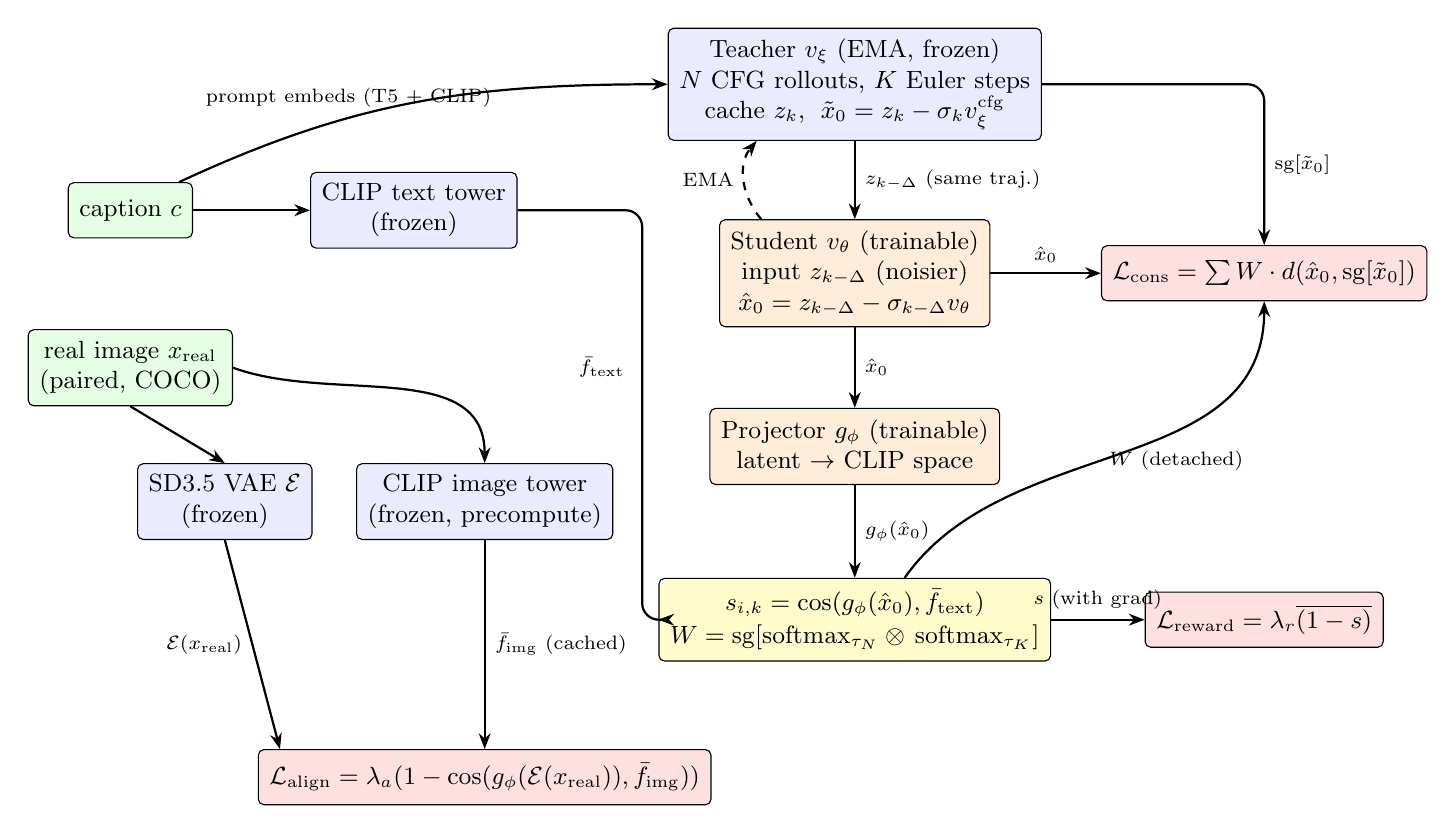
\begin{tikzpicture}[
  font=\small,
  box/.style={draw, rounded corners=2pt, align=center, inner sep=4pt, minimum height=7mm},
  frozen/.style={box, fill=blue!8},
  train/.style={box, fill=orange!15},
  data/.style={box, fill=green!10},
  loss/.style={box, fill=red!12},
  scorebox/.style={box, fill=yellow!20},
  arr/.style={-{Stealth[length=2mm]}, thick},
  dashedarr/.style={arr, dashed},
  lab/.style={font=\scriptsize},
]

% ── Center chain: teacher → student → projector → score ──
\node[frozen] (teacher) at (9.2, 7.2)
  {Teacher $v_\xi$ (EMA, frozen)\\$N$ CFG rollouts, $K$ Euler steps\\
   cache $z_k$,\; $\xtil = z_k - \sigma_k v^{\mathrm{cfg}}_\xi$};
\node[train] (student) at (9.2, 4.8)
  {Student $v_\theta$ (trainable)\\input $z_{k-\Delta}$ (noisier)\\
   $\xhat = z_{k-\Delta} - \sigma_{k-\Delta} v_\theta$};
\node[train] (proj) at (9.2, 2.6)
  {Projector $g_\phi$ (trainable)\\latent $\to$ CLIP space};
\node[scorebox] (score) at (9.2, 0.4)
  {$s_{i,k} = \cossim(g_\phi(\xhat), \ftext)$\\[1pt]
   $W = \sg[\mathrm{softmax}_{\tau_N} \otimes\, \mathrm{softmax}_{\tau_K}]$};

% ── Left column: inputs and frozen encoders ──
\node[data] (caption) at (0, 5.6) {caption $c$};
\node[frozen] (cliptext) at (3.6, 5.6) {CLIP text tower\\(frozen)};
\node[data] (image) at (0, 3.6) {real image $x_{\mathrm{real}}$\\(paired, COCO)};
\node[frozen] (vae) at (1.2, 1.9) {SD3.5 VAE $\mathcal{E}$\\(frozen)};
\node[frozen] (clipimg) at (4.5, 1.9) {CLIP image tower\\(frozen, precompute)};

% ── Right column: losses ──
\node[loss] (lcons) at (14.4, 4.8)
  {$\mathcal{L}_{\mathrm{cons}} = \sum W \cdot d(\xhat, \sg[\xtil])$};
\node[loss] (lreward) at (14.4, 0.4)
  {$\mathcal{L}_{\mathrm{reward}} = \lambda_r \overline{(1-s)}$};
\node[loss] (lalign) at (4.5, -1.6)
  {$\mathcal{L}_{\mathrm{align}} = \lambda_a (1 - \cossim(g_\phi(\mathcal{E}(x_{\mathrm{real}})), \fimg))$};

% ── Center chain edges ──
\draw[arr] (teacher) -- node[right, lab] {$z_{k-\Delta}$ (same traj.)} (student);
\draw[arr] (student) -- node[right, lab] {$\xhat$} (proj);
\draw[arr] (proj) -- node[right, lab] {$g_\phi(\xhat)$} (score);
\draw[dashedarr] (student.150) to[out=130, in=230]
  node[left, lab] {EMA} (teacher.210);

% ── Caption conditioning ──
\draw[arr] (caption) -- (cliptext);
\draw[arr] (caption.30) to[out=25, in=180]
  node[above, lab, pos=0.35] {prompt embeds (T5 + CLIP)} (teacher.west);
% f_text wire: down the empty corridor between encoder and center columns
\draw[arr, rounded corners=6pt]
  (cliptext.east) -- (6.5, 5.6) -- (6.5, 0.4) -- (score.west);
\node[lab, left] at (6.4, 3.6) {$\ftext$};

% ── Losses: consistency ──
\draw[arr] (student.east) -- node[above, lab] {$\xhat$} (lcons.west);
\draw[arr, rounded corners=6pt] (teacher.east) -| 
  node[right, lab, pos=0.75] {$\sg[\xtil]$} (lcons.north);
\draw[arr] (score.40) to[out=55, in=270]
  node[right, lab, pos=0.45] {$W$ (detached)} (lcons.south);

% ── Losses: reward ──
\draw[arr] (score.east) -- node[above, lab] {$s$ (with grad)} (lreward.west);

% ── Losses: projector anchor ──
\draw[arr] (image.south) -- (vae.north);
\draw[arr] (image.east) to[out=-20, in=90] (clipimg.north);
\draw[arr] (vae.south) -- node[left, lab] {$\mathcal{E}(x_{\mathrm{real}})$}
  ($(lalign.north)+(-2.6,0)$);
\draw[arr] (clipimg.south) -- node[right, lab] {$\fimg$ (cached)}
  (lalign.north);

\end{tikzpicture}%
}
\caption{v5 components. Green: data; blue: frozen; orange: trainable;
yellow: scoring; red: loss terms. The teacher generates trajectories and
Tweedie targets; the student predicts $\xhat$ from noisier states of the same
trajectories; the projector scores $\xhat$ against the caption's CLIP text
embedding $\ftext$, producing both the detached Boltzmann weights $W$ and the
differentiable reward. The real image is used only to anchor the projector
($\mathcal{L}_{\mathrm{align}}$). The dashed EMA arrow closes the
self-distillation loop.}
\label{fig:components}
\end{figure}

\section{Implementation Details}

\begin{table}[h]
\centering
\small
\begin{tabular}{@{}llp{7.2cm}@{}}
\toprule
\textbf{Component} & \textbf{Value} & \textbf{Notes} \\
\midrule
Base model & SD3.5-Medium (2.5B MMDiT) & flow matching; velocity prediction \\
Encoder & CLIP ViT-L/14 (\texttt{openai}) & projected (joint-space) embeddings, $d = 768$ \\
Data & COCO \texttt{train2017} captions & 591{,}753 (image, caption) pairs; $\fimg$ cached once \\
Trajectories & $N = 4$, $K = 8$ Euler steps & CFG $\omega = 7.0$ (batched uncond$\Vert$cond) \\
Scoring window & $[0.4, 0.9] \cdot K \Rightarrow k \in \{3, \dots, 7\}$ & mid-to-late noise band \\
Timestep gap & $\Delta \sim \mathcal{U}\{1, 3\}$, one per $k$ & student always noisier than target \\
Temperatures & $\tau_N = \tau_K = 1.0$, z-scored $s$ & max traj.\ weight ${\approx}0.5$ at $N{=}4$; lower $\tau$ to sharpen \\
Loss weights & $\lambda_r = 1.0$, $\lambda_a = 1.0$ & \\
Distance & pseudo-Huber, $c = 0.00054\sqrt{D} \approx 0.14$ & MSE available as ablation \\
EMA decay & $m = 0.999$ & fp32 EMA (bf16 increments round to zero) \\
Precision & fp32 master weights, bf16 autocast & student, teacher, projector all fp32 \\
Optimizer & AdamW, $\beta = (0.9, 0.999)$ & two param groups \\
LR (student) & $1 \times 10^{-5}$, linear warmup 500 & pretrained-model fine-tuning scale \\
LR (projector) & $1 \times 10^{-4}$ & random init; REPA's projector LR \\
Grad clip & student 1.0, projector 5.0 & clipped separately \\
Batching & 1 caption/rank/step; pass 2 is one $|\mathcal{K}| N{=}20$ forward & gradient checkpointing on \\
Hardware & $4 \times$ H200 (141 GB), DDP & rank-disjoint prompt streams (DistributedSampler) \\
Steps & 150{,}000; checkpoint every 500 & wandb: losses, $s$, $W$ entropies, EMA samples \\
\bottomrule
\end{tabular}
\caption{v5 configuration.}
\end{table}

\section{Design Choices}

\begin{itemize}
\item \textbf{Consistency in $x_0$ space, not feature space.} The matched
quantity ($\xhat$) has a fixed meaning at every timestep, so there is no
constant-feature collapse mode, and the full network --- including the
velocity readout --- sits in the gradient path. Pseudo-Huber follows iCT/LCM
practice.
\item \textbf{Asymmetric gap direction.} Student at higher noise matching a
lower-noise target along the same teacher trajectory mirrors consistency
distillation's adjacent-pair structure (with $\Delta$ playing the role of
LCM's skipping step), transferring late-trajectory information to earlier
timesteps.
\item \textbf{CFG-mixed Tweedie targets.} Distilling the \emph{guided}
prediction (guidance distillation) bakes prompt adherence into the
single conditional student forward and keeps the target consistent with the
states the rollout actually visits.
\item \textbf{Detached Boltzmann weights.} $\mathrm{softmax}(s/\tau)$ is a
Gibbs distribution with energy $-s$; treating $W$ as a constant is the
correct reward-weighted-regression form. Backpropagating through the weights
would create pressure to \emph{reduce} alignment on hard pairs.
\item \textbf{Text-embedding scoring.} $s$ approximates CLIPScore --- the
actual prompt-alignment quantity. Scoring against the paired image's
embedding would instead impose single-image reconstruction (captions are
many-to-many).
\item \textbf{Projector as cheap reward proxy.} No VAE decode and no CLIP
vision forward in the training loop; the projector amortizes both. Its
faithfulness is maintained by $\mathcal{L}_{\mathrm{align}}$ on real-image
latents (clean targets, REPA-style), preventing reward hacking via projector
collapse.
\item \textbf{fp32 masters + fp32 EMA.} With $m = 0.999$, EMA increments are
$\sim\!10^{-3} (\theta - \xi)$ --- below bf16 resolution. All trainable and
EMA parameters are fp32; compute runs under bf16 autocast.
\item \textbf{Score standardization.} Per-axis z-scoring of $s$ before the
softmaxes decouples the weighting's selectivity from the projector's output
scale and from CLIP's compressed cosine range; without it the Boltzmann
weights are empirically near-uniform ($W$ entropy pinned at
$\log(N|\mathcal{K}|)$).
\item \textbf{Known limitations (tracked).} (i) The projector anchor is
trained on clean latents but scores Tweedie predictions (domain gap);
(ii) the loop has no real-data term for the \emph{student} --- drift is
monitored via periodic EMA-teacher samples.
\end{itemize}

\end{document}
